\documentclass{article}

\title{Indeksowa organizacja pliku}
\author{Dominik Lau (188697)}

\usepackage{blindtext}
\usepackage{amsmath}
\usepackage[utf8]{inputenc}
\usepackage[polish]{babel}
\usepackage[T1]{fontenc}
\usepackage{listings}
\usepackage{color}
\usepackage{amssymb}
\usepackage{esvect}
\usepackage{graphicx}
\usepackage{mathtools}
\usepackage[margin=0.5in]{geometry}
\DeclarePairedDelimiter\ceil{\lceil}{\rceil}
\DeclarePairedDelimiter\floor{\lfloor}{\rfloor}

\graphicspath{ {./obrazy/} }

\definecolor{dkgreen}{rgb}{0,0.6,0}
\definecolor{gray}{rgb}{0.5,0.5,0.5}
\definecolor{mauve}{rgb}{0.58,0,0.82}
\def\multiset#1#2{\ensuremath{\left(\kern-.3em\left(\genfrac{}{}{0pt}{}{#1}{#2}\right)\kern-.3em\right)}}

\lstset{frame=tb,
  language=C++,
  aboveskip=3mm,
  belowskip=3mm,
  showstringspaces=false,
  columns=flexible,
  basicstyle={\small\ttfamily},
  numbers=none,
  numberstyle=\tiny\color{gray},
  keywordstyle=\color{blue},
  commentstyle=\color{dkgreen},
  stringstyle=\color{mauve},
  breaklines=true,
  breakatwhitespace=true,
  tabsize=3
}


\begin{document}
\maketitle

\section{Wprowadzenie}
Celem projektu była implementacja indeksowo-sekwencyjnej organizacji pliku z mozliwością dodawania, usuwania i aktualizacji rekordów, a następnie zbadanie 
wpływu parametrów na działanie tej struktury.
Wylosowane przeze mnie typy rekordów to \textbf{numery rejestracyjne samochodów}. Implementacji
dokonałem w języku C++.
\section{Opis działania}
\subsection{Struktura kodu}
W moim rozwiązaniu stosuję:
\begin{itemize}
\item klasy rekordów indeksu i pliku z danymi, udostępniające narzędzia do serializacji
\item klasę \textit{File} z pliku \textit{generic/File.h} zawierającą implementację
pliku dyskowego o dostępie blokowym,  która obsługuje logikę zapisu/odczytu stron z pliku dyskowego tak,że
dostęp do niego poprzez metody \textit{get} czy \textit{insert} są na podobieństwo dostępu do zwykłej tablicy w pamięci RAM. Struktura ta cache'uje strony, odczytuje i zapisuje tylko w przypadku konieczności jej wymiany (ponadto zapis następuje tylko w przypadku modyfikacji ``bitu`` \textit{dirty} na true)
 \item klasę \textit{IndexedFile} udostępniającą m.in. metody \textit{remove, insert, update, reorganise} (o których więcej w następnch podpunktach)
 \item folder \textit{cli/} zawierający ``agenty`` - \textit{InteractiveAgent, RandomAgent, FileAgent} definiujące źródło wejścia do programu, odpowiednio z wiersza poleceń, losowe oraz z pliku
\item folder \textit{time/} zawierający zegary i klasy pomiarowe do zliczania operacji dyskowych
\end{itemize}
\subsection{Serializacja/deserializacja}
Rekordy z pliku indeksowego składają się z dwóch 4-bajtowych pól (numer strony i klucz), których kolejne bajty umieszczam w pliku zgodnie z konwencją little endian. W przypadku rekordu z danymi mamy trzy pola do serializacji - klucz, wskaźnik na następny rekord w obszarze przepełnienia (jeśli następny taki rekord nie znajduje
się w obszarze przepełnienia, to pole to ma wartość \textbf{0xFFFFFFFF}) oraz \textbf{7-bajtowe pole z danymi}.  W przypadku, gdy rozmiar strony nie jest równy wielokrotności rozmiaru rekordu, reszta jest uzupełniana bajtami 0xFF.
\subsection{Operacje na pliku indeksowym}
\begin{itemize}
\item tworzenie (konstruktor) - oferuje możliwość podania liczby stron głównych do stworzenia, ilość
	stron przeznaczonych na obszar przepełnienia to $\ceil{\text{il.  stron głównych} * 0.2}$. \textbf{Na początku działania programu tworzony jest plik o 3 stronach głównych} (a co za tym idzie jednej stronie na obszar przepełnienia).
\item insert - wstawienie nowego rekordu - pierw algorytmem binary search \textbf{przeszukujemy indeks} w poszukiwaniu odpowiedniego bloku,  następnie \textbf{przeszukujemy blok w poszukiwaniu poprzednika} wstawianego klucza, jeśli nie możemy wstawić rekordu bezpośrednio za poprzednikiem (np. już jest tam jakiś rekord lub strona jest pełna),  \textbf{umieszczamy go w łańcuchu przepełnienia tego rekordu} , jeśli obszar przepełnienia jest pełny, przeprowadzamy reorganizację pliku indeksowego
\item reorganise 
\begin{enumerate}
	\item tworzymy tymczasowy plik indeksowy z indeksami \textit{temp\_index i temp\_data}, z których plik data ma ilość głównych stron zgodną ze wzorem $\ceil{\frac{N+V}{b\cdot\alpha}}$,  gdzie $N,V$ - liczba odpowiednio  rekordów głównych i rekordów w przepełnieniu, $b$ - liczba rekordów danych na stronę, $\alpha$ - średnie zapełnienie strony po reorganizacji
 plik tymczasowy index ma odpowiednią liczbę stron tak, żeby zmieścić wskaźniki do wszystkich stron nowego obszaru głównego
	\item \textbf{odwiedzamy kolejne rekordy zgodnie z kolejnością rosnących kluczy} (czyli bierzemy też po uwagę obszar przepełnienia) i umieszczamy je na kolejnych stronach nowego pliku respektując przy tym $\alpha$
	\item zmieniamy pliki \textit{temp\_index i temp\_data} na \textit{data i index},  w ten sposób dane po reorganizacji przypisujemy do pliku indeksowego, na którym operujemy
	\item zastosowano tu optymalizację związaną z faktem, że w mojej implementacji strony są cache'owane i zapisywane tylko wtedy, gdy to konieczne (w sposób lazy) - tworzę osobny bufor na strony z obszaru przepełnienia, wówczas mam jednocześnie cache stron obszaru głównego i overflow i  nie zachodzi potrzeba ciągłego ich wymieniania
\end{enumerate}
\item remove - znalezienie odpowiedniego miejsca w strukturze i usunięcie z niego rekordu, tutaj na miejsce, w którym był ten rekord ``wciągamy`` następny z łańcucha przepełnienia (jeśli taki występuje)
\item update - \textbf{jeśli chcemy aktualizować klucz} dla danego rekordu to najpierw usuwamy go z pliku a następnie wstawiamy na nowo ze zmodyfikowanymi danymi; \textbf{jeśli aktualizujemy tylko dane} to pobieramy pozycję rekordu o danym kluczu i zmieniamy jego numer rejestracyjny
\end{itemize}
\section{Prezentacja wyników programu}
\subsection{Menu wyboru źródła danych}
Po włączeniu programu użytkownik ma do wyboru trzy tryby
\begin{lstlisting}
[INFO] debug mode false
CHOOSE INPUT TYPE: CLI/FILE/RANDOM, set/unsets DEBUG
\end{lstlisting}
\begin{itemize}
	\item CLI - tryb interaktywny
	\item FILE <nazwa\_pliku> - dane z pliku o podanej nazwie
	\item RANDOM <N> - generacja losowej ilości poleceń (INSERT/REMOVE/UPDATE)
	\item DEBUG - włączenie wypisywania stanu pliku co każdą operację
\end{itemize}
Po zakończeniu dla każdego z tych plików użytkownik ma możliwość wypisania końcowej postaci pliku.
\subsection{Menu interaktywne}
Menu oferuje następujące komendy
\begin{lstlisting}
>>HELP
INSERT <key> <value>
REMOVE <key>
UPDATE <key> <newKey> <newValue>
GET <key>
REORGANISE
INORDER
EXIT
\end{lstlisting}
komenda INORDER oferuje wypisanie pliku zgodnie z kolejnością kluczy,
oto przykładowe wywołanie komendy INSERT z wyłączonym trybem debug
\begin{lstlisting}
>>INSERT 3 GS2138
[Measurement] r: 1 w: 0 io(r+w): 1
\end{lstlisting}
Otrzymujemy informacje o wykonanych zapisach i odczytach (0 zapisów, ponieważ rekord jest narazie w cache'u, 1 odczyt ponieważ strona z pliku indeksowego najwyraźniej nadal jest w cache).
\subsection{Dane z pliku}
Plik, z którego pobierane są dane musi zawierać instrukcje w formacie takim, jak w przypadku menu interaktywnego, ponadto każda musi być w osobnej linii. Ciąg instrukcji kończyć musi instrukcja EXIT.
\subsection{Wypisywanie pliku}
Są dwa sposoby, w jaki program wypisuje plik, pierwszy - wypisanie struktury pliku razem z pustymi miejscami i zaznaczeniem jaki rekord jest na której stronie, oto przykład
\begin{lstlisting}
___INDEXED__FILE___
-------INDEX-------
=======PAGE0======
page: 0 key: 0
page: 1 key: 98852148
page: 2 key: 198206151
-----INDEX-END-----

------PRIMARY------
=======PAGE0======
#0 key: 0 data: BRUUUUH ptr: 14
#1 key: 68030329 data: DEBUG69
#2 *******************
#3 *******************
=======PAGE1======
#4 key: 98852148 data: 4O353I3
#5 *******************
#6 *******************
#7 *******************
=======PAGE2======
#8 key: 198206151 data: P5MP165
#9 *******************
#10 *******************
#11 *******************
----PRIMARY-END----

-----OVERFLOW------
=======PAGE0======
#12 key: 68030327 data: BUP30QP ptr: 13
#13 key: 68030328 data: DEBUG70
#14 key: 35496734 data: K7302PD ptr: 12
#15 *******************
----OVERFLOW-END---
\end{lstlisting}
a oto wypisanie tego samego pliku zgodnie z kolejnością klucza
\begin{lstlisting}
___INDEXED__FILE___
#0 key: 0 data: BRUUUUH
#14 key: 35496734 data: K7302PD
#12 key: 68030327 data: BUP30QP
#13 key: 68030328 data: DEBUG70
#1 key: 68030329 data: DEBUG69
#4 key: 98852148 data: 4O353I3
#8 key: 198206151 data: P5MP165
\end{lstlisting}

\section{Eksperyment}
\subsection{Szczegóły implementacyjne}
Kod przeprowadzonego eksperymentu umieściłem w pliku \textit{perf2.cpp} jako część biblioteki \textit{sbd\_test}. Test uruchamiany jest za pomocą frameworka do
testowania gtest. W celu zliczania operacji wejścia-wyjścia w \textit{libsbd} zdefiniowałem dwa zegary: 
\textit{writeClock} oraz \textit{readClock}. W pomiarach wykorzystuję również klasę \textit{Measurement}, która zbiera próbki na wzór paradygmatu RAII - w 
konstruktorze zapisywany jest aktualny stan zegara a w destruktorze nowy stan zegara jest odejmowany od starego, w ten sposób otrzymuję liczbę
wywołań funkcji \textit{tick} danego zegara. Ponadto pomiary te dodawane są do obiektu klasy \textit{MeasurementAggregate}, który umożliwia policzenie wartości średniej z zebranych próbek. \\\\
\textbf{W przypadku testów przyjęto rozmiar strony 750B}.
\subsection{Rozmiar a ilość rekordów}
Pierwszym przeprowadzonym eksperymentem było zbadanie zależności między liczbą rekordów a rozmiarem pliku.  W tym celu przyjęto $\alpha = 0.5$ i przeprowadzono $N$ losowych operacji INSERT.
\begin{center}
\begin{tabular}{ c | c c c | c}
 $N$ & rozmiar indeksu [B] & rozmiar obszaru głównego [B] & rozmiar obszaru przepełnienia [B] & $\Sigma$ [B]  \\ 
\hline
  50 & 750 & 2250 & 750 & 3750 \\
  250 & 750 & 5250 & 1500 & 7500 \\
  500  & 750 & 12750 & 3000 & 16500 \\
  1000 & 750 & 29250 & 6000 & 36000 \\
  2500 & 750 & 58500 &  12000 & 71250 \\
  5000 & 1500 & 118500 & 24000 & 144000 \\
  7500 & 2250 & 161250 & 32250 & 195750 \\
  10000 & 3000 & 236250 & 47250 & 286500\\
\end{tabular}
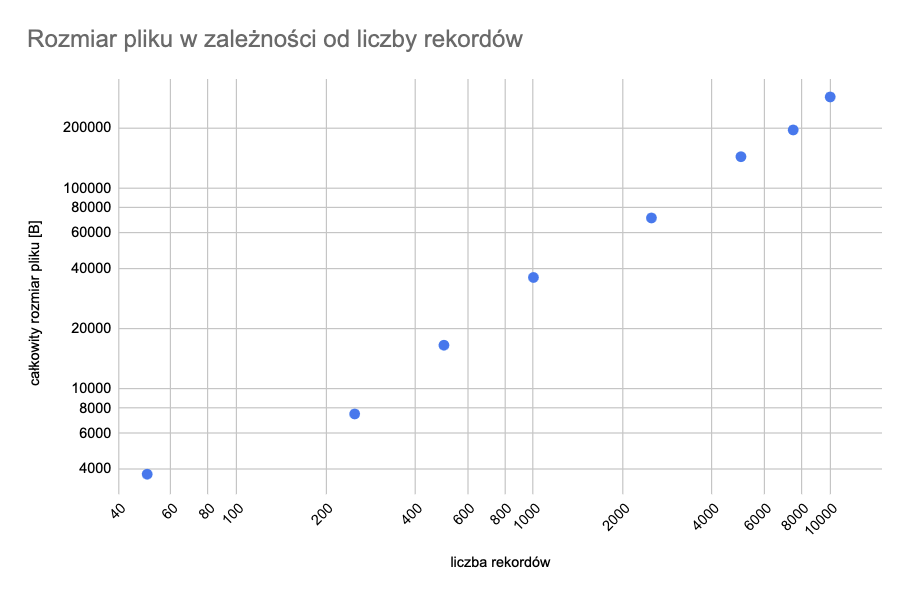
\includegraphics[width=10cm]{rozmiar_rekordy}
\end{center}
Intuicyjnie, \textbf{całkowity rozmiar pliku indeksowego rośnie liniowo względem liczby rekordów}.  Warto natomiast zwrócić uwagę na rozmiar indeksu, który rośnie znacznie wolniej - dla 10000 rekordów ma on zaledwie 3000B czyli 4 strony. Stąd
wniosek, że \textbf{opłacalnym jest przeszukiwanie indeksu} zarówno ze względu na jego mały rozmiar jak i na fakt, że jedna strona indeksu zawiera informacje o wielu stronach w obszarze danych.
\subsection{Rozmiar a $\alpha$}
W następnym eksperymencie przeprowadzono 1000 losowych operacji INSERT dla różnych współczynników średniego zapełnienia bloku i zbadano końcowy rozmiar pliku
\begin{center}
\begin{tabular}{ c | c c c | c}
 $\alpha$ & rozmiar indeksu [B] & rozmiar obszaru głównego [B] & rozmiar obszaru przepełnienia [B]  & $\Sigma$ [B] \\ 
\hline
  0.1 & 1500 & 120000 & 24000 & 145500 \\
   0.2 & 750 & 62250 & 12750 & 75750 \\
  0.3 & 750 & 34500 & 7500 & 42750 \\
  0.4 & 750 & 33750 & 6750 & 41250 \\
  0.5 & 750 & 28500 & 6000 & 35250 \\
  0.6 & 750 & 25500 & 5250 & 31500 \\
  0.7 & 750 & 17250 & 3750 & 21750 \\
  0.8 & 750 & 18000 & 3750 & 22500 \\
  0.9 & 750 & 16500 & 3750 & 21000 \\
\end{tabular}
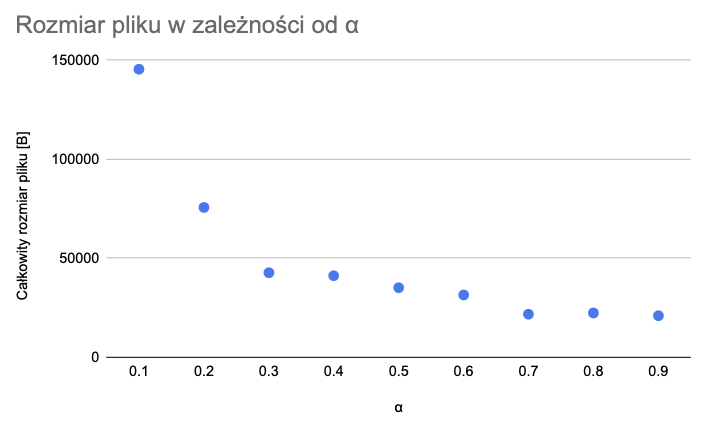
\includegraphics[width=10cm]{rozmiar_alfa}
\end{center}
Warto zauważyć, że dla $\alpha \in [0.1,0.3]$ następuje \textbf{gwałtowny spadek rozmiaru pliku}. Dalej tendencja się utrzymuje jednak w mniejszym stopniu. Czym większe $\alpha$, tym \textbf{reorganizacja utworzy mniej stron (które będą bardziej ``upchane``)}. Potencjalnym wytłumaczeniem, dlaczego tendencja spadkowa się osłabia jest np. \textbf{częstsze zachodzenie
reorganizacji} wraz ze wzrostem $\alpha$ (szybsze zapełnianie się stron, mniejszy obszar przepełnienia). Wysnuć mozna wniosek, że chcąc zaoszczędzić pamięć dyskową, opłaca się wybrać większe $\alpha$. 
\subsection{Średnia liczba operacji dla różnych $\alpha$}
W kolejnym eksperymencie  wygenerowano 1000 losowych rekordów z kluczami $\in [0, 1000]$, sprawdzono złożoność dla wstawiania, a następnie badano średnią ilość odczytów/zapisów dla 100 operacji aktualizacji, usuwania i szukania (i ich różnych przypadków)
dla $\alpha \in \{0.1, 0.3, 0.5\}$. 
\begin{center}
\textbf{dla} $\alpha = 0.1$ \\
\begin{tabular}{ c | c c | c}
 operacja & średnia liczba odczytów & średnia liczba zapisów & średnia liczba operacji i/o \\ 
\hline
 wstawianie & 3.95 & 2.21 & 6.16 \\  
 \hline 
 \textbf{rekord istnieje}\\
 aktualizacja (inny klucz) &  5.98 & 3.41 & 9.39 \\
 aktualizacja (ten sam k.) & 2.45 & 1.00 & 3.45 \\
 usunięcie & 2.91 & 1.52 & 4.43 \\
 szukanie & 2.45 & 0.01 & 2.46\\
 \hline
 \textbf{rekord nie istnieje} \\
 aktualizacja (inny klucz) & 2.53 & 0.01 & 2.54 \\
 aktualizacja (ten sam k.) & 2.35 & 0.01 & 2.36\\
 usunięcie & 2.35 & 0.01 & 2.36\\
 szukanie & 2.35 & 0.01 & 2.36 \\
\hline \hline
\end{tabular}
\end{center}
\begin{center}
\textbf{dla} $\alpha = 0.3$ \\
\begin{tabular}{ c | c c | c}
 operacja & średnia liczba odczytów & średnia liczba zapisów & średnia liczba operacji i/o \\ 
\hline
 wstawianie & 2. 957& 2.019 & 4.976 \\  
 \hline 
 \textbf{rekord istnieje}\\
 aktualizacja (inny klucz) &  4.97 & 2.76 & 7.73 \\
 aktualizacja (ten sam k.) & 1.32 & 0.99 & 2.31 \\
 usunięcie & 2.08 & 0.93 & 3.01 \\
 szukanie & 1.32 & 0.01 & 1.33 \\
 \hline
 \textbf{rekord nie istnieje} \\
 aktualizacja (inny klucz) & 1.8 & 0.01 & 1.81\\
 aktualizacja (ten sam k.) & 1.75 & 0.01 & 1.76\\
 usunięcie  & 1.75 & 0.01 & 1.76\\
 szukanie & 1.75 & 0.01 & 1.76\\
\hline \hline
\end{tabular}
\end{center}
\begin{center}
\textbf{dla} $\alpha = 0.5$ \\
\begin{tabular}{ c | c c | c}
 operacja &średnia liczba odczytów & średnia liczba zapisów & średnia liczba operacji i/o \\ 
\hline
 wstawianie & 3.018 & 2.064 & 5.082 \\  
 \hline 
 \textbf{rekord istnieje}\\
 aktualizacja (inny klucz) & 3.46 & 2.76 & 6.22 \\
 aktualizacja (ten sam k.) & 1.05 & 0.96 & 2.01 \\
 usunięcie & 1.21 & 0.9 & 2.11 \\
 szukanie & 1.05 & 0.01 & 1.06\\
 \hline
 \textbf{rekord nie istnieje} \\
 aktualizacja (inny klucz) & 1.1 & 0.01 & 1.11 \\ 
 aktualizacja (ten sam k.) & 1.06 & 0.01 & 1.07 \\
 usunięcie & 1.06 & 0.01 & 1.07\\
 szukanie & 1.06 & 0.01 & 1.07 \\
\hline \hline 
\end{tabular}
\end{center}
Dla $\alpha=0.1$ obserwujemy większą ilośc operacji niż dla pozostałych - dzieje się tak ponieważ mamy większą ilość stron a zatem i częściej zachodzą przypadki takie jak konieczność wymiany strony (odwołanie do strony, która nie znajduje się w pamięci cache), dla dużego $\alpha$ natomiast jest większe prawdopodobieństwo, że w kolejnej operacji nastąpi odwołanie do strony, którą akurat trzymamy w pamięci operacyjnej.  Nie należy jednak wyciągać pochopnych wniosków - ta różnica może być zaniedbywalnie mała dla ogromnej ilości stron.  Ponadto, \textbf{są to róznice do dwóch operacji dyskowych}. \\\\
Jeśli chodzi o same operacje to widzimy, że\textbf{ najbardziej złożona jest operacja update ze zmianą klucza}.
Choć w implementacji sprowadza się do wywołania remove a następnie insert to w średnim przypadku trwa mniej niż suma tych operacji ze względu na \textbf{obecność pamięci cache}.  W przypadku aktualizacji danych rekordu, mamy do czynienia ze znacznie szybszą metodą (wówczas jest to znalezienie odpowiedniego rekordu i ponowne zapisanie go ze zmienionymi danymi).  Pragnę również zauważyć, że w przypadku \textbf{gdy rekord nie istnieje operacje aktualizacji, usunięcia i szukania wymagają podobnej ilości dostępów} do dysku.
\section{Podsumowanie}
Reasumując, projekt pozwolił na głębsze zrozumienie organizacji indeksowej pliku a także ich własności. 
Z eksperymentów płynie uzasadnienie,  dlaczego w tej strukturze używany jest indeks - umożliwia on szybkie przeszukiwanie pliku. Można poczynić również obserwacje co do rozmiaru plików w zależności od tego jak przeprowadzamy reorganizację pliku (czym większe $\alpha$ tym mniejszy plik). W końcu, eksperymenty potwierdziły oczekiwania co do wzajemnego stosunku średniej ilości I/O dla poszczególnych operacji.



\end{document}
